\chapter{Simulation results}

In this chapter we shall present a collection of the most interesting results obtained to validate the numerical performance of discretization method described in the previously chapters. 

\section{Test cases}


We focus our tests over three kind of semiconductor devices: 

\begin{itemize}
\item {\bf p-n junction}
\item {\bf p-n junction in oxide}
\item {\bf MOS n-channel}
\end{itemize}

For everyone of these case test we shall investigate the correction of the FEMOS solution against the results obtained with SDEVICE.  


\subsection{p-n junction}

In this example we consider a p-n junction also known as diode. In \figref{fig: diodo struttura} we present the partition used and the doping profile of this test case. The section of the parallelepiped is a $0.05 \times 0.05 [\mu m^2]$ square while the device is $0.1 [\mu m]$ long.  The number of verticises used is $4933$.  The doping concentration is obtained setting a constant profile of acceptor over all the domain ($N_A = 1.0\times 10^{17}$) overhelmed by a doping profile of acceptor ($N_D=1.0 \times 10^{18}$) bounded on one side of the device. As you can see we defined the two different areas of doping with an almost abrupt junction. 
Two contacts are defined, then on the first (A) is applyed a voltage of $0.3[V]$ while the opposite one (B) is grounded. In this situation the diode is direct polarized. The  relative electric permettivity of the silicon is $\epsilon_{SI} = 11.6 [F cm^{-1}]$ while the mobility model used is the thermal model \referenzaeq{eq: mobility thermal} with a constant temperature of $300 [K]$.

\begin{figure}[!t]
\centering
\subfloat[][\emph{Mesh}]
{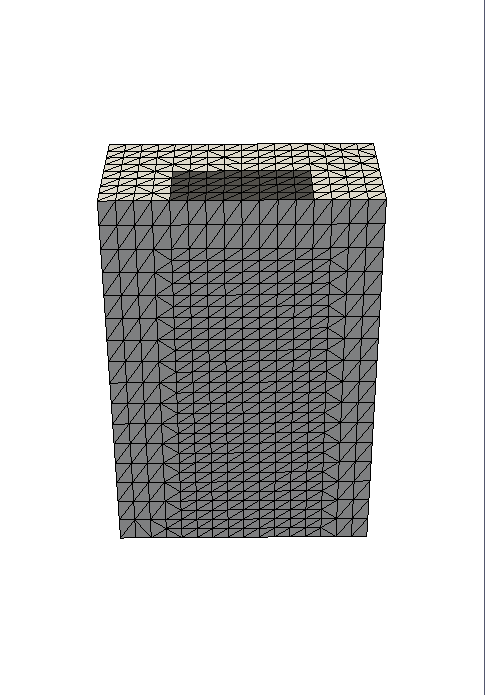
\includegraphics[scale=0.43]{Results/DIODE/AAA_structureandcontact.png}}
\hspace{0.5cm}
\subfloat[][\emph{Doping concentration $[cm^{-3}]$}]
{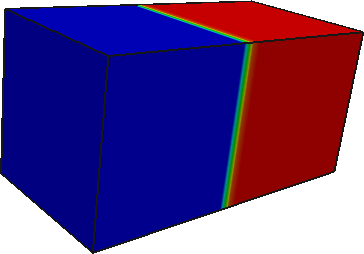
\includegraphics[scale=0.43]{Results/DIODE/AAA_DopingconcentrationONLYDEVICE.png}}
\hspace{0.5cm}
\subfloat[][]
{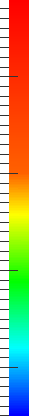
\includegraphics[scale=0.3]{Results/MOS/LegendaArcobalenoVert.png}}
\caption{Test case diode p-n.}
\label{fig: diodo struttura}
\end{figure}


In \ref{fig: diode potential}, \ref{fig: ndensity} and \ref{fig: pdensity} we validated FEMOS results against SDEVICE. As we aspected from theory the drop in potential is almost bounded around the junction, and as we use an asymmetric doping, it is major extended on the p-side. Notice that on the minority contact, which means A contact for electron solution and B contact for hole solution, the Dirichlet condition causes a big drop in concetration (from $1.0\times 10^{15}$ to $1.0 \times 10^3$ $[cm^{-3}]$) \textcolor{red}{qua introduco questo commento per legarmi poi ai problemi che abbiamo riscontrato nel conto della corrente}. 

Now we are interested to analyze the computational performance of this numerical scheme. We know that the main difficulty is the initialization of the variables and obiouvsly the convergence time is strictly related to the kind of initial step we use. However predict in every situations the possibly shape of the solutions is hard, if not even impossible. For this reason a common and general approach is used: we split the domain in several regions accordingly to their doping concentration. Once obtained this partition we treat every of those semiconductor regions as they are in equilibrium with the nearest contact. This hypotesis allow us to compute over the entire domain the initial step for $\varphi$, $n$ and $p$ thanks to the relations \referenzaeq{eq: non eq n density mb} and \referenzaeq{eq: non eq p density mb}. 
Even this choice of initial step some difficulties may occur, especially if we consider the device far away the equilibrium condition. We can state this effect looking at the figure \figref{fig: tempi computazionali}, where computational costs are shown against the polarization. We notice that at $1.0[V]$ the computational time increase really quickly, and then it remains stable.  
This voltage level is almost the $built-in$ of this p-n junction, which means ....

\begin{figure}[!h]
\centering
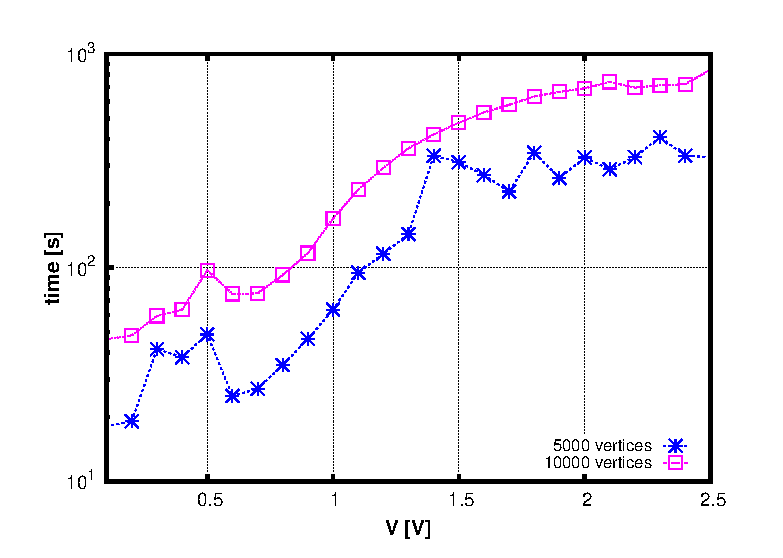
\includegraphics[scale=0.8]{Results/Caratteristiche/Diode/ComputationalTimeDifferentMeshes.eps}
\caption{Computational times for different bias in two mesh cases.}
\label{fig: tempi computazionali}
\end{figure}

The graph \figref{fig: times and iterations} shows us that this problem is related to the convergence of the Gummel Map and not to the shape of the system matrix of the equations. Indeed while the number of iterations increase like the curve of total time computation, the times refer to the computational time of NLP and DD solver equation remain stable.

\begin{figure}[!h]
\centering
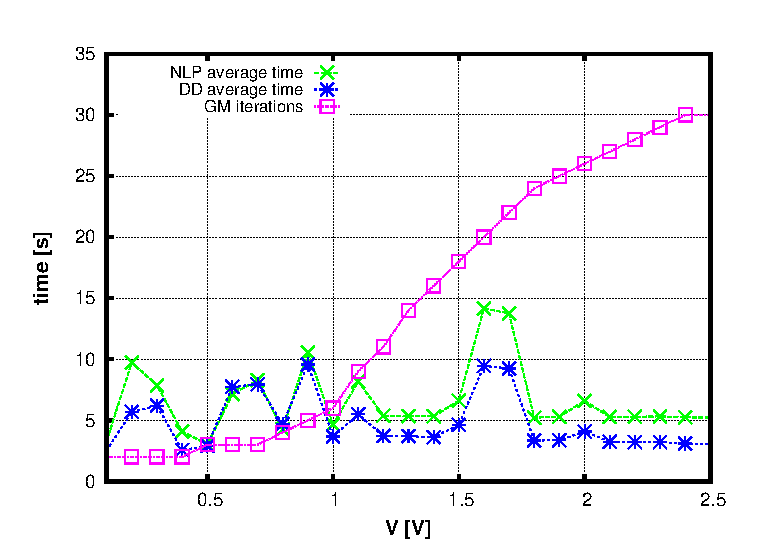
\includegraphics[scale=0.8]{Results/Caratteristiche/Diode/ConfrontoTempiNLPDDGMiterations.eps}
\caption{Computational times and iterations.}
\label{fig: times and iterations}
\end{figure}



We can see that the shape of the solutions after the buil-in level are really different from the initial step \textcolor{red}{referenza figura plot over line del potenziale}.

\begin{figure}[!h]
\centering
\subfloat[][]
{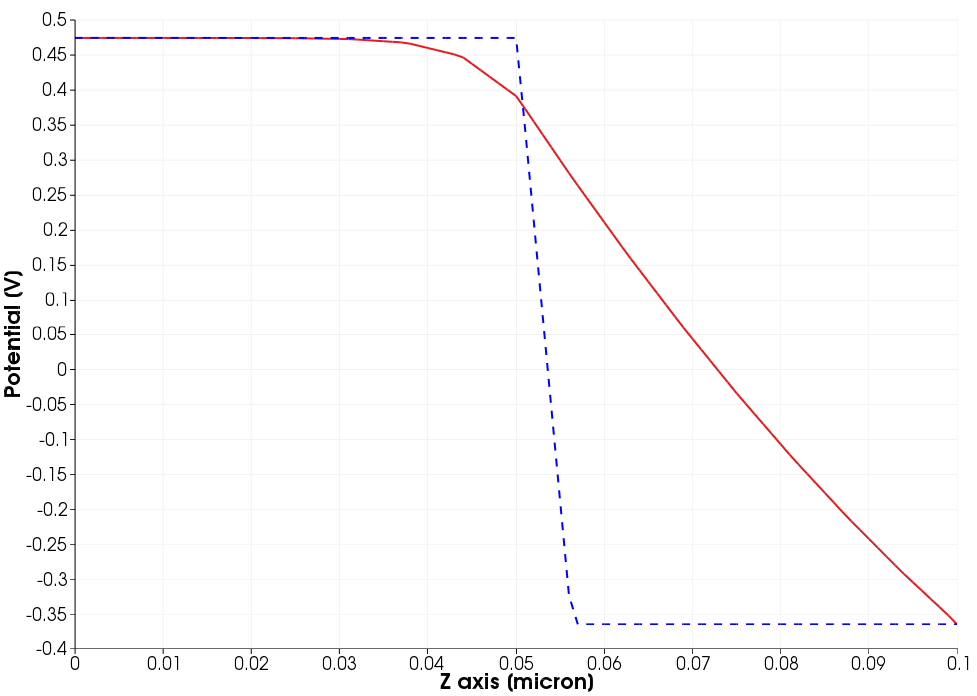
\includegraphics[scale=0.18]{Results/PlotOverLine/Diode/InitialGuess01volt.png}}
\hspace{1cm}
\subfloat[][]
{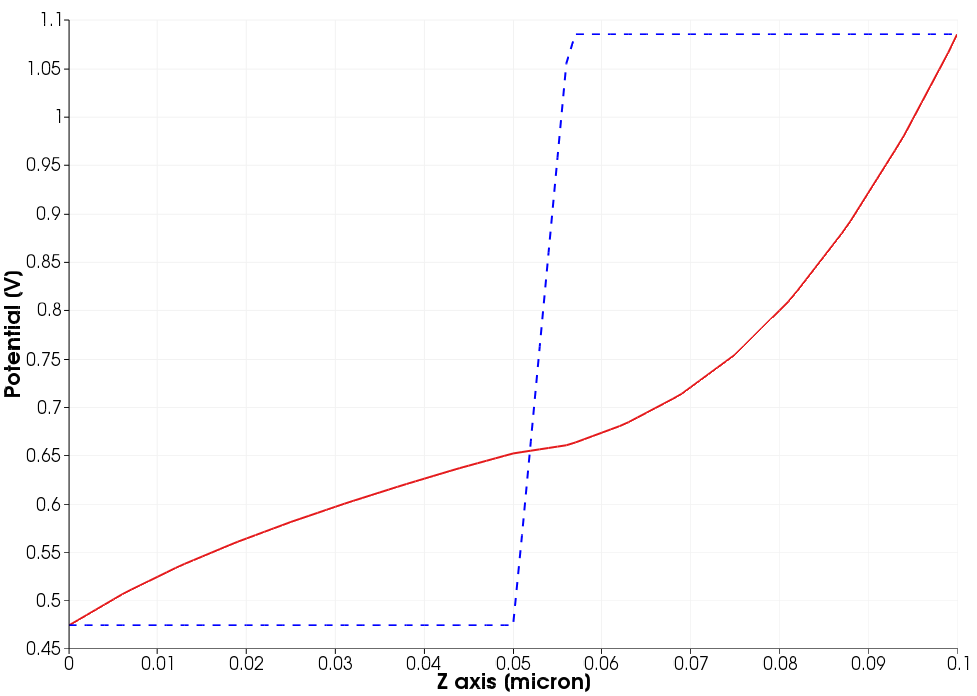
\includegraphics[scale=0.18]{Results/PlotOverLine/Diode/InitialGuess15volt.png}}
\end{figure}

So if we are far away from the equilbrium ...
Il sistema e fuori dall'equilibrio le soluzioni differiscono molto dalla soluzione iniziale


\begin{figure}[!h]
\centering
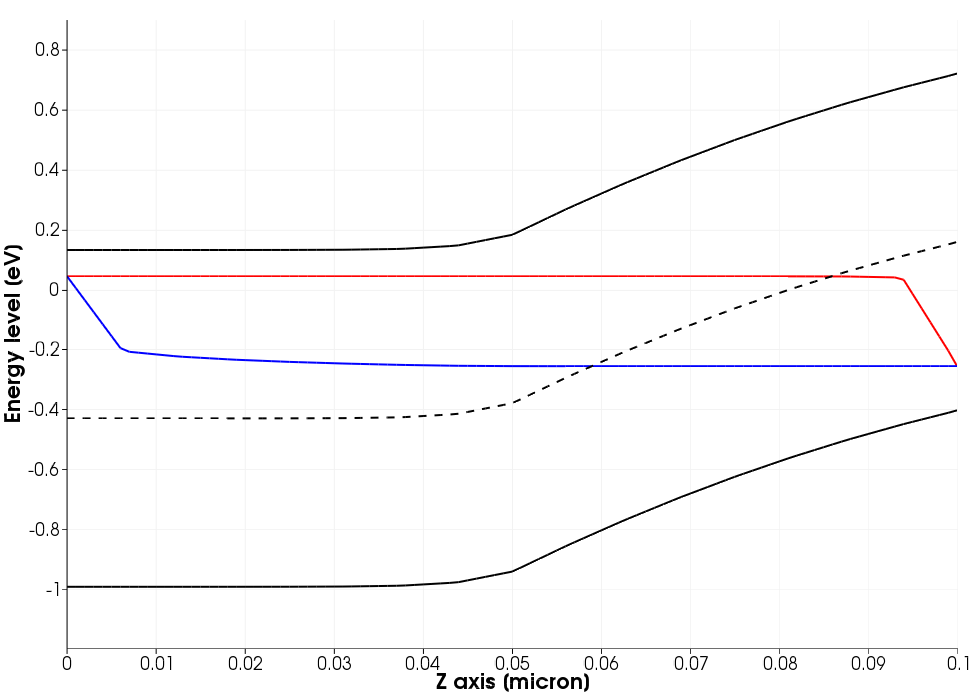
\includegraphics[scale=0.25]{Results/PlotOverLine/Diode/Bande03volt}
\end{figure}


\clearpage 

\begin{figure}[!h]
\centering
\subfloat[][\emph{FEMOS}]
{\includegraphics[scale=0.43]{Results/DIODE/FEMOS1817_potential03volt.png}}
\hspace{0.5cm}
\subfloat[][]
{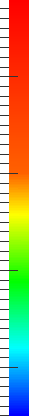
\includegraphics[scale=0.3]{Results/MOS/LegendaArcobalenoVert.png}}
\hspace{0.5cm}
\subfloat[][\emph{SDEVICE}]
{\includegraphics[scale=0.43]{Results/DIODE/SDEVICE1817_potential03voltONLYDEVICE.png}}
\caption{Test case dide p-n 0.3[V] potential.}
\label{fig: diode potential}
\end{figure}

\begin{figure}[!h]
\centering
\subfloat[][\emph{FEMOS}]
{\includegraphics[scale=0.43]{Results/DIODE/FEMOS1817_edensity03volt.png}}
\hspace{0.5cm}
\subfloat[][]
{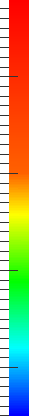
\includegraphics[scale=0.3]{Results/MOS/LegendaArcobalenoVert.png}}
\hspace{0.5cm}
\subfloat[][\emph{SDEVICE}]
{\includegraphics[scale=0.43]{Results/DIODE/SDEVICE1817_edensity03voltONLYDEVICE.png}}
\caption{Test case dide p-n 0.3[V] electron density.}
\label{fig: ndensity}
\end{figure}

\begin{figure}[!h]
\centering
\subfloat[][\emph{FEMOS}]
{\includegraphics[scale=0.43]{Results/DIODE/FEMOS1817_hdensity03volt.png}}
\hspace{0.5cm}
\subfloat[][]
{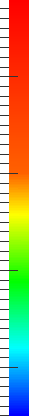
\includegraphics[scale=0.3]{Results/MOS/LegendaArcobalenoVert.png}}
\hspace{0.5cm}
\subfloat[][\emph{SDEVICE}]
{\includegraphics[scale=0.43]{Results/DIODE/SDEVICE1817_hdensity03voltONLYDEVICE.png}}
\caption{Test case dide p-n 0.3[V] hole density.}
\label{fig: pdensity}
\end{figure}


\clearpage


\subsection{p-n junction in oxide}

In this test case we surrounded the previous structure with a layer of oxide material ($\epsilon_{ox} = 3.9 [F cm^{-1}]$). This layer is about $0.025[\mu m]$ thick and notice that the contacts are defined only on the silicon region. As the physical behaviour in the oxide is much less complicated than in the semiconductor part, we chose to use a smaller step of discretization in this zone. We spent $6334$ verticies overall the domain. The structure and the doping are well defined in \figref{fig: structure diodeox}. The setting of the electrode is the same of the previously simulation. We still validate our solutions with the commercial software in \figref{fig: potential diodeox}, \figref{fig: edensity diodeox} and \figref{fig: hdensity diodeox}.  



\begin{figure}[!h]
\centering
\subfloat[][\emph{Mesh}]
{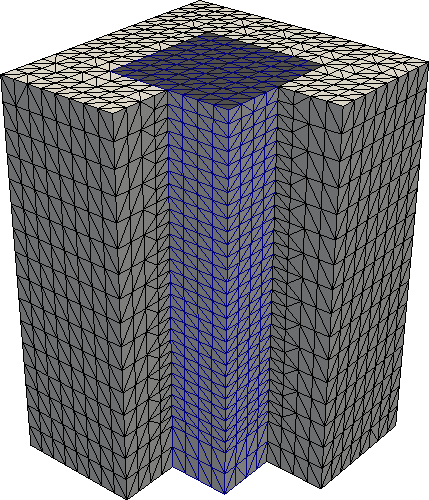
\includegraphics[scale=0.3]{Results/DIODEOX/AAA_structureandcontact2.png}}
\hspace{1.5cm}
\subfloat[][\emph{Doping concentration}]
{\includegraphics[scale=0.3]{Results/DIODEOX/AAA_Dopingconcentration2ONLYDEVICE.png}}
\caption{Test case p-n junction in oxide.}
\label{fig: structure diodeox}
\end{figure}


It's interesting notice the behaviour of the potential inside the oxide layer, indeed it seems to be more diffused than in the silicon. This phenomena is clear if we think about the relation \referenzaeq{eq: relazione pot electric} between electric field and potential.
 As we imposed $\nabla \varphi \cdot \vect{n}=0$ on the oxide boundary no field lines of the electric field could cross that boundary. The conseguence is that all the field lines could start and end only from the contact A or B.
Therefore the behaviour of the the electric field inside the device is due only to the displacement effect on the junction of the silicon, which imposes the electric response in the oxide material, see \figref{fig: electric field diode}. The conseguence is a lower electric field in the oxide which implies a more diffused potential.
We remind that the electric field variable is post-processed by the electric potential, this is a conseguence of adopting a displacement formulation approach.

\begin{figure}[!t]
\centering
\subfloat[][\emph{FEMOS}]
{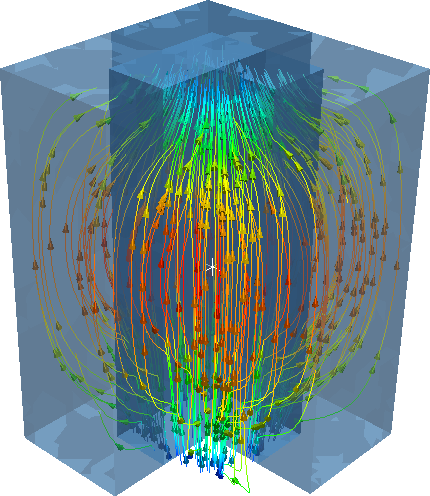
\includegraphics[scale=0.35]{Results/DIODEOX/FEMOS1817_electricfield03volt.png}}
\hspace{1.5cm}
\subfloat[][\emph{SDEVICE}]
{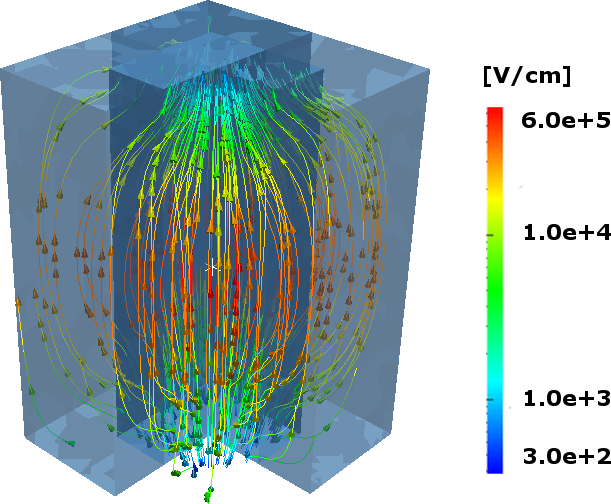
\includegraphics[scale=0.35]{Results/DIODEOX/SDEVICE1817_electricfield03voltONLYDEVICE.png}}
\caption{Test case dide p-n in ox 0.3[V], electric field.}
\label{fig: electric field diode}
\end{figure}

\begin{figure}[!h]
\centering

\subfloat[][]
{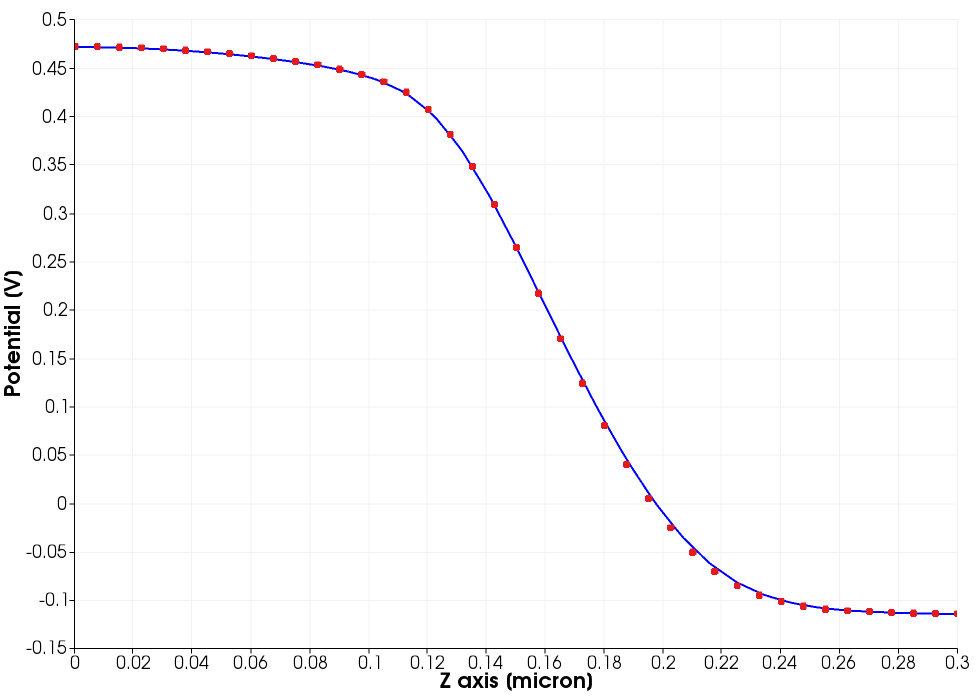
\includegraphics[scale=0.18]{Results/PlotOverLine/DiodeOx/Potential03voltLOW}}
\hspace{1cm}
\subfloat[][]
{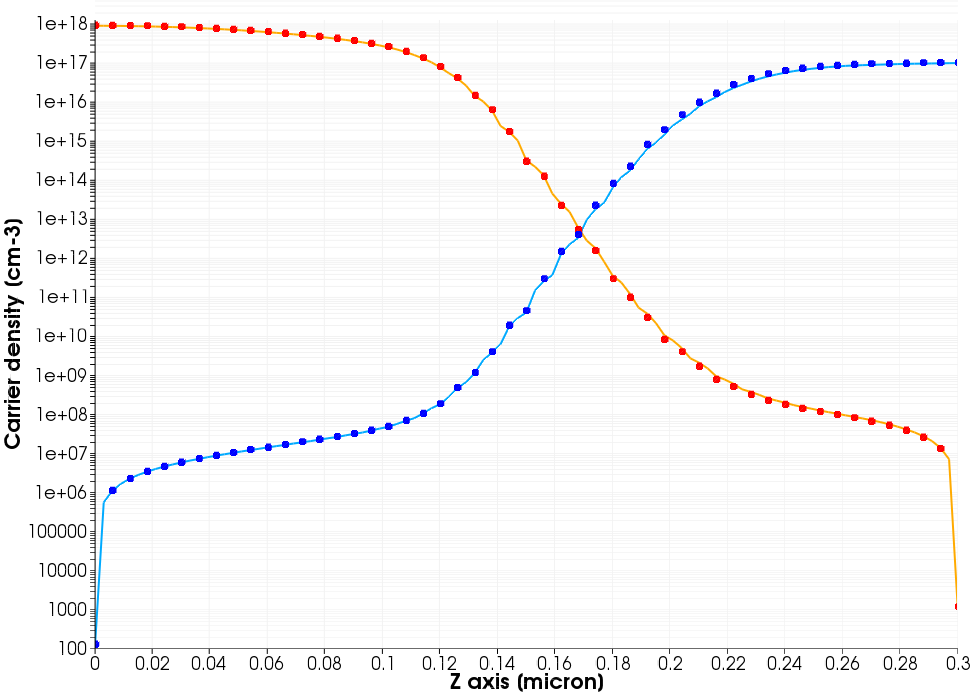
\includegraphics[scale=0.18]{Results/PlotOverLine/DiodeOx/CarriersDensity03volt}}

\subfloat[][]
{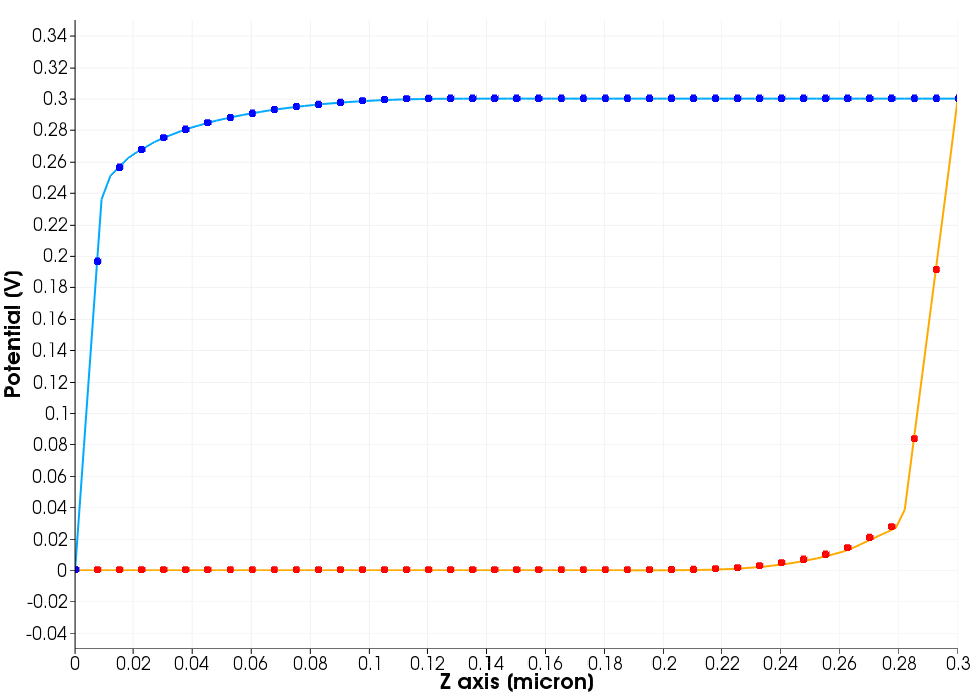
\includegraphics[scale=0.18]{Results/PlotOverLine/DiodeOx/QuasifermiPot03volt}}


\end{figure}




\clearpage


\begin{figure}[!h]
\centering
\subfloat[][\emph{FEMOS}]
{\includegraphics[scale=0.26]{Results/DIODEOX/FEMOS1817_potential03volt.png}}
\hspace{1cm}
\subfloat[][\emph{SDEVICE}]
{\includegraphics[scale=0.26]{Results/DIODEOX/SDEVICE1817_potential03voltONLYDEVICE.png}}
\caption{Test case dide p-n in ox 0.3[V].}
\label{fig: potential diodeox}
\end{figure}

\begin{figure}[!h]
\centering
\subfloat[][\emph{FEMOS}]
{\includegraphics[scale=0.26]{Results/DIODEOX/FEMOS1817_edensity03volt.png}}
\hspace{1cm}
\subfloat[][\emph{SDEVICE}]
{\includegraphics[scale=0.26]{Results/DIODEOX/SDEVICE1817_edensity03voltONLYDEVICE.png}}
\caption{Test case dide p-n in ox 0.3[V].}
\label{fig: edensity diodeox}
\end{figure}

\begin{figure}[!h]
\centering
\subfloat[][\emph{FEMOS}]
{\includegraphics[scale=0.26]{Results/DIODEOX/FEMOS1817_hdensity03volt.png}}
\hspace{1cm}
\subfloat[][\emph{SDEVICE}]
{\includegraphics[scale=0.26]{Results/DIODEOX/SDEVICE1817_hdensity03voltONLYDEVICE.png}}
\caption{Test case dide p-n in ox 0.3[V].}
\label{fig: hdensity diodeox}
\end{figure}

\clearpage









\subsection{MOSFET n-channel}

The functionality of a \textit{MOSFET} device is quite complex, therefore we give a summary of its basic operation. For a more detailed description see \textcolor{red}{referenza per mos}.
The metal-oxide-semiconductor field-effect transistor (MOSFET) is the building block of VLSI circuits in microprocessors and dynamic memories. Because the current in a MOSFET is transported predominantly by carriers of one polarity, the MOSFET is usually referred to as a unipolar or majority-carrier device.
In this test case we consider an \textit{n-channel MOSFET} or \textit{nMOSFET} which consists of a p-type silicon substrate into which two n-regions are formed. 
Its structure is well defined in \figref{fig: mos geometry}. It is a four-terminal device with the electrodes designated as gate (G), source (S), drain (D) and substrate or bulk (B). The gate electrode is usually made of metal or heavily doped polysilicon and is separated from the substrate by a thin silicon dioxide. The surface region under the gate  oxide between source and drain is called the \textit{channel} region.
We describe briefly the basic operation of a MOSFET device.
When there is no voltage applied to the gate there is no current flow between the source and drain, while if a sufficiently large positive voltage is applied to the gate, the silicon surface is inverted to n-type, which forms a conducting channel between the source and drain. In the latter case if we apply a voltage to the drain the electrons start to flow from source to drain and therefore a current in the opposite direction is generated. 
As we know already where the phenomena shall be more interesting we performed an oriented meshing which is high fitted along the channel region, at the contact and over the deplation region \figref{fig: mos geometry}. The n-regions are implanted accordingly with a gaussian profile.


\vspace{1cm}

\begin{figure}[!h]
\centering
\subfloat[][\emph{Mesh}]
{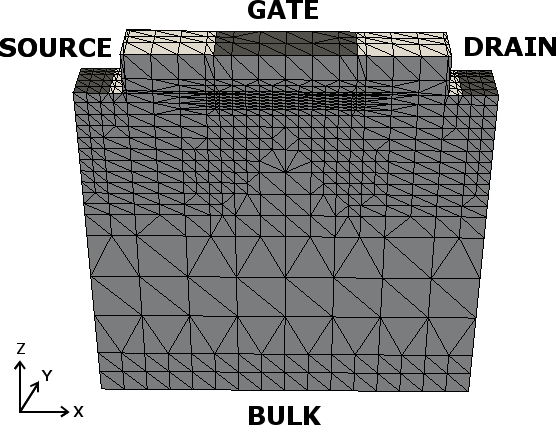
\includegraphics[scale=0.37]{Results/MOS/AAA_MeshAndContact.png}}
\hspace{1cm}
\subfloat[][\emph{Doping concentration}]
{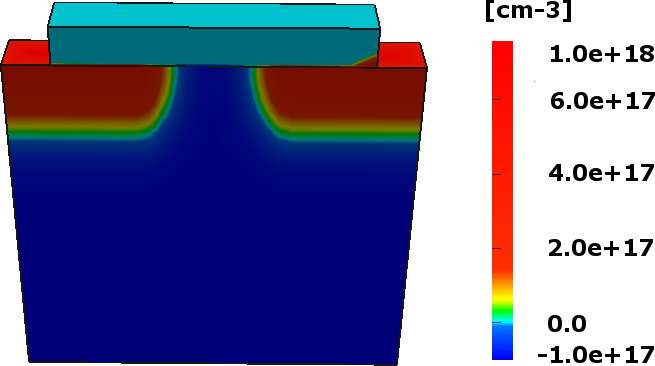
\includegraphics[scale=0.37]{Results/MOS/AAA_DopingConcentrationONLYDEVICE.png}}
\hspace{0.5cm}
\subfloat[][]
{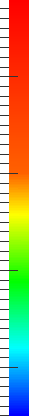
\includegraphics[scale=0.3]{Results/MOS/LegendaArcobalenoVert.png}}
\caption{Geometry of the test case MOS n-channel.}
\label{fig: mos geometry}
\end{figure}


We match our result in the operating phase of the MOSFET, therefore the setting of the electrode is $V_G=2.0[V]$, $V_D=0.1[V]$ and $V_S=V_B=0.0[V]$. The results are shown in \ref{fig: potential mos}, \figref{fig: ndensity mos} and \figref{fig: pdensity mos}. Whereas the channel region is a p-region, with this polarization its nature is changed to an n-region, for better understand the formation of the channel see \textcolor{red}{ref figura equilibrio} which represents the electron and hole density of the same device for a $V_G=0.0[V]$.

\begin{figure}[!h]
\centering
\subfloat[][]
{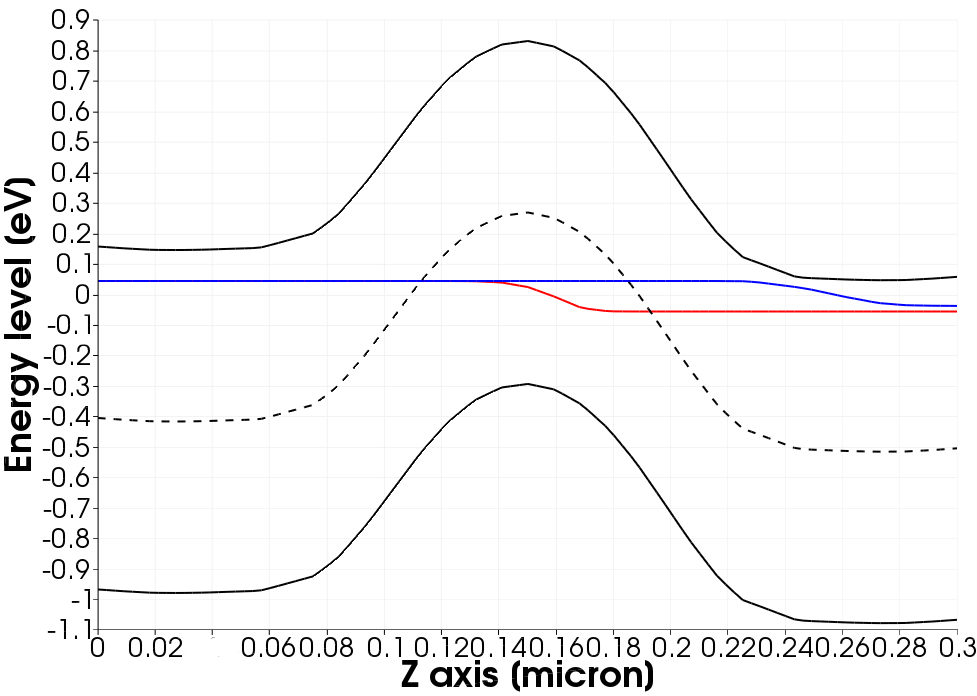
\includegraphics[scale=0.3]{Results/PlotOverLine/Mos/BandLevels0volt}}

\subfloat[][]
{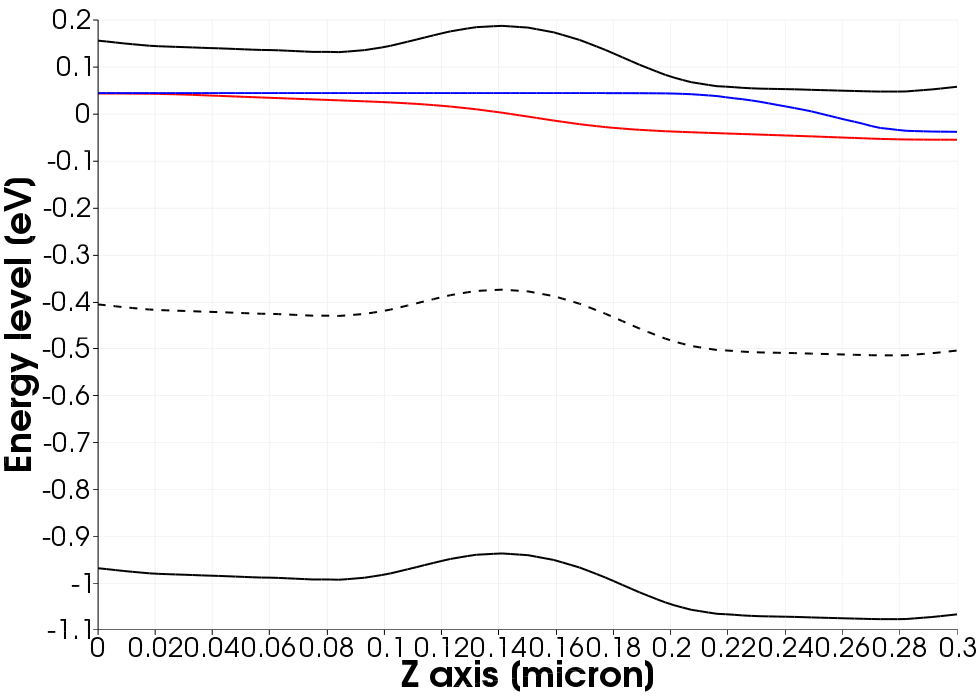
\includegraphics[scale=0.3]{Results/PlotOverLine/Mos/BandLevels2volt}}
\end{figure}


\begin{figure}[!h]
\centering
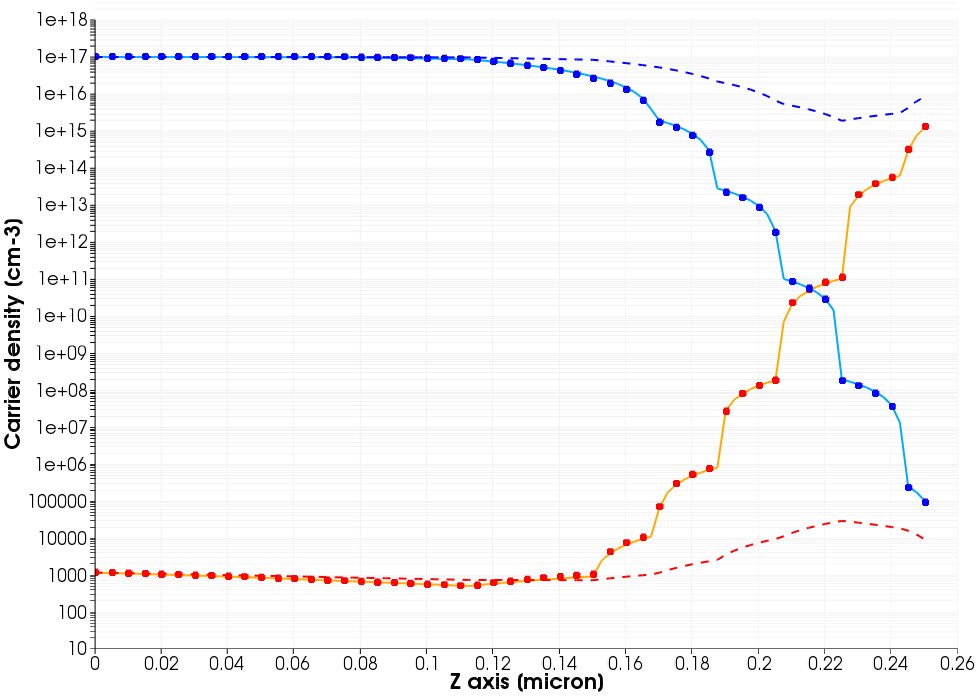
\includegraphics[scale=0.3]{Results/PlotOverLine/Mos/ChargeSheet1_5to2}
\end{figure}

\begin{figure}[!h]
\centering
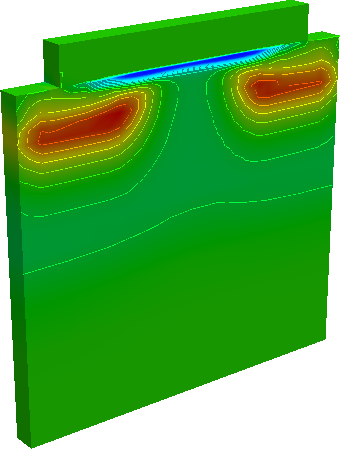
\includegraphics[scale=0.45]{Results/PlotOverLine/Mos/Contour3DSpacechargeONLYDEVICE}
\caption{Space charge $V_G=2.0[V]$}
\end{figure}



\clearpage

\begin{figure}[!h]
\centering
\subfloat[][\emph{FEMOS}]
{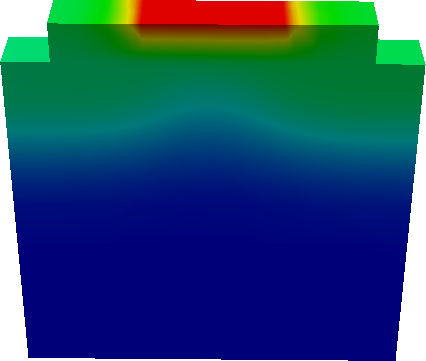
\includegraphics[scale=0.37]{Results/MOS/FEMOS181718_potential2voltONLYDEVICE.png}}
\hspace{0.5cm}
\subfloat[][]
{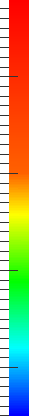
\includegraphics[scale=0.3]{Results/MOS/LegendaArcobalenoVert.png}}
\hspace{0.5cm}
\subfloat[][\emph{SDEVICE}]
{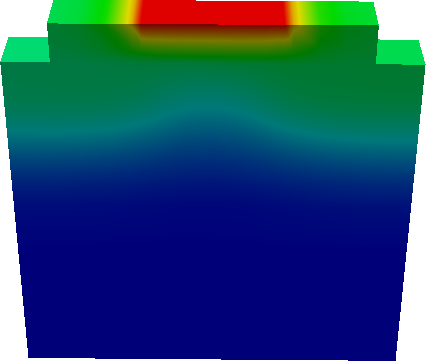
\includegraphics[scale=0.37]{Results/MOS/SDEVICE181718_potential2voltONLYDEVICE.png}}
\caption{Potential Vgate = 2.0 [V].}
\label{fig: potential mos}
\end{figure}


\begin{figure}[!h]
\centering
\subfloat[][\emph{FEMOS}]
{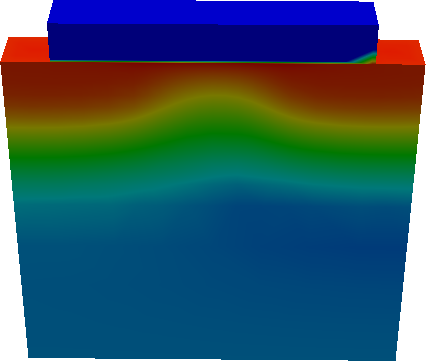
\includegraphics[scale=0.37]{Results/MOS/FEMOS181718_ndensity2voltONLYDEVICE.png}}
\hspace{0.5cm}
\subfloat[][]
{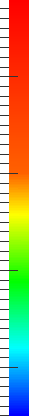
\includegraphics[scale=0.3]{Results/MOS/LegendaArcobalenoVert.png}}
\hspace{0.5cm}
\subfloat[][\emph{SDEVICE}]
{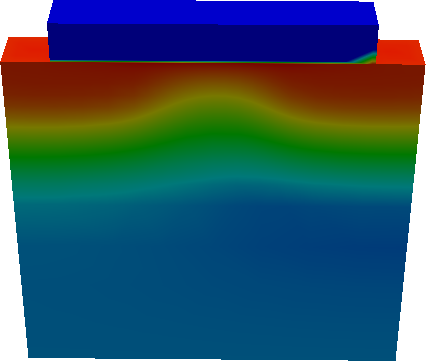
\includegraphics[scale=0.37]{Results/MOS/SDEVICE181718_ndensity2voltONLYDEVICE.png}}
\caption{Electron density Vgate = 2.0 [V].}
\label{fig: ndensity mos}
\end{figure}

\begin{figure}[!h]
\centering
\subfloat[][\emph{FEMOS}]
{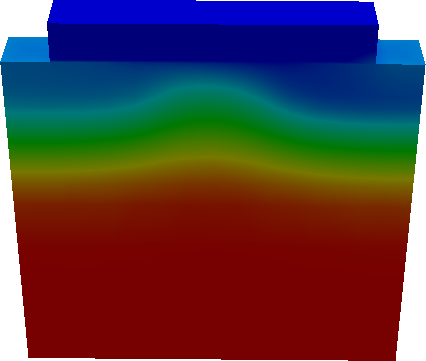
\includegraphics[scale=0.37]{Results/MOS/FEMOS181718_pdensity2volt.png}}
\hspace{0.5cm}
\subfloat[][]
{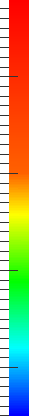
\includegraphics[scale=0.3]{Results/MOS/LegendaArcobalenoVert.png}}
\hspace{0.5cm}
\subfloat[][\emph{SDEVICE}]
{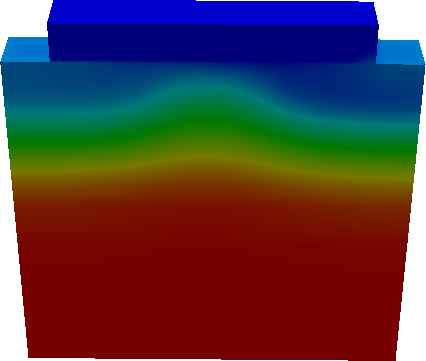
\includegraphics[scale=0.37]{Results/MOS/SDEVICE181718_pdensity2voltONLYDEVICE.png}}
\caption{Electron density Vgate = 2.0 [V].}
\label{fig: pdensity mos}
\end{figure}



Show how decade the GCA the gradual channel approzimation which assumes that the variation of the electric field along the channel is much less than the corresponding variation in the orthogonal direction (perpendicular to the channel).

\begin{figure}[!h]
\centering
\subfloat[][\emph{FEMOS}]
{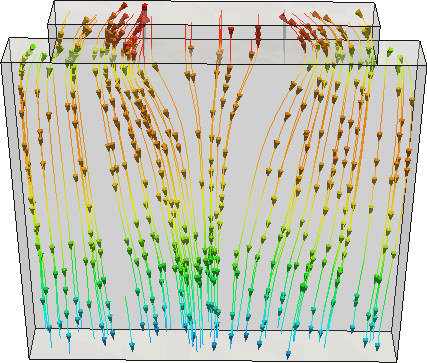
\includegraphics[scale=0.38]{Results/MOS/FEMOS181718_ElectricField2voltONLYDEVICE.png}}
\hspace{0.5cm}
\subfloat[][]
{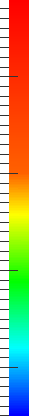
\includegraphics[scale=0.3]{Results/MOS/LegendaArcobalenoVert.png}}
\hspace{0.5cm}
\subfloat[][\emph{SDEVICE}]
{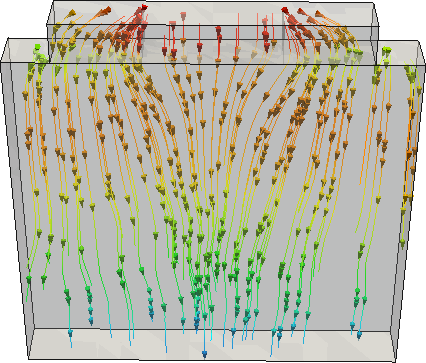
\includegraphics[scale=0.38]{Results/MOS/SDEVICE181718_ElectricField2voltONLYDEVICE.png}}
\caption{Electric field density Vgate = 2.0 [V].}
\end{figure}

\clearpage


\section{Current at contacts}

During the analysis of an electric device, one of the most useful information is the electrical response at terminals. In order to accomplish this target we have to compute the integral of the electron and hole current density over a generic electrode.
Consider $\Gamma_{D,Si} = \bigcup_{i=1}^d \Gamma_i$ where $d$ is the number of terminals on the device and $\forall i=1,...,d$ $\Gamma_i$ is the $i$-th contact. The problem is $\forall i$ compute:

\begin{equation}
\mathcal{I}_i = \mathcal{I}_i^n + \mathcal{I}_i^p
\end{equation}

where $\mathcal{I}_i$ is the total current, $\mathcal{I}_i^n$ is the contribution of the electron current and $\mathcal{I}_i^p$ is the contribution of the hole current.
In general, given a contact $\Gamma_i$, fluxes of current density to be calculated assume the following form:

\begin{equation}
\label{eq: current flux}
\mathcal{I}_i^\nu = \int_{\Gamma_i}\vect{J}_\nu(\nu) \cdot \vect{n} \, d{\Gamma_i} \psp{10} \nu = \{n,p\}
\end{equation}

where as usual $\vect{n}$ is the unit outward normal of the domain boundary. It's well known that the evaluation of boundary integrals is a difficult task. Many difficulties in the numerical evalutaion of \referenzaeq{eq: current flux} arise from singularities in spatial derivatives of the approximate solution $n^h$ or $p^h$ near the contact edges, due to a change in the boundary condition type (e.g. from Dirichlet to Neumann) at the contact ends.

In the following we present an accurate method for the evaluation of boundary integrals in semiconductor device based on the work \cite{ContactCurrentRM}, we shall extend the \textit{residue method} to the 3D case and we confirm the optimal results matching them with SDEVICE. Moreover we remark that the method can be succesfully applied to a wide spread of applications, including contact charges, carrier quantum probability fluxes and heat fluxes.

Before go further with the presentation of the results, it's useful look up the anlysis made in \cite{ContactCurrentRM} and adapt it to our case. Let be $A$ the system matrix of the continuity equation \referenzaeq{eq: matrice continuità} and $\vect{b}$ the relative right hand side before applying boundary conditions.  The linear problem looks as:

\begin{equation}
\label{eq: discretization before bc}
\sum_{j\in\eta} A_{ij} \nu_j = b_i \psp{10} \forall i \in \eta
\end{equation}

where $\eta$ is the set of all vertices of the partition $\mathcal{T}_h$, $\nu_j$ is the generic $j$-th component of the carrier solution.  We can split the set of total nodes in contact node $\eta_g$ and the complementary part $\eta_n$.
Notice that the values of $\nu_j$ are known on the contacts and \referenzaeq{eq: discretization before bc} can be rewritten as follows:

\begin{equation}
\label{eq: discretization before bc 2}
\begin{cases}

\sum_{j\in\eta_n} A_{ij} \nu_j = b_i - \sum_{j\in\eta_g} A_{ij} \nu_j & \forall i \in \eta_n \\
\\
\sum_{j\in\eta_n} A_{ij} \nu_j = b_i - \sum_{j\in\eta_g} A_{ij} \nu_j & \forall i \in \eta_g \\

\end{cases}
\end{equation}

The first set of equations is the usual linear system which we solve while the second can be used for boundary flux estimation. 
 Now we define a new test function $v^h_i$ as:

\begin{equation}
\label{eq: new test function}
v^h_i=\sum_{j\in\eta_{gi} }\psi_j
\end{equation}

where $\eta_{gi}$ is the set of nodes lying on $\Gamma_i$. Substituting \referenzaeq{eq: new test function} in \referenzaeq{eq: current flux} we can estate that:

\begin{multline}
\mathcal{I}_i^\nu 
= \int_{\Gamma_i}\vect{J}_\nu(\nu) \cdot \vect{n} \, d{\Gamma_i}
= \sum_{j=1}^{n_d}\int_{\Gamma_j}\vect{J}_\nu(\nu) \cdot \vect{n} \,v_i^h \, d{\Gamma_j} \\
=\sum_{i\in\eta_{gi}}\sum_{j=1}^{n_d}\int_{\Gamma_j}\vect{J}_\nu(\nu) \cdot \vect{n} \, \psi_i \, d{\Gamma_j} 
= \sum_{i\in \eta_{gi}}\int_{\partial \Omega}\vect{J}_\nu(\nu) \cdot \vect{n} \, \psi_i \, d{\partial \Omega} \\
= \sum_{i\in \eta_{gi}} \left[ \int_{\Omega}\nabla \cdot \vect{J}_\nu(\nu) \psi_i \, d{\Omega} + \int_{\Omega}\vect{J}_\nu(\nu) \cdot \nabla\psi_i \, d{\Omega} \right] \\
= \sum_{m\in \eta_{gi}} \left[ \sum_{j\in\eta} A_{ij} \nu_j\psi_i - b_i  \right] \\
\end{multline}

The current at contact $i$ is performed by summing the residuals of the matrix $A$.

Per questo è detto metodo dei residui ...

Nel seguito mostriamo alcuni risultati ...

\subsection{Results}

We shall apply the residue method over all the devices presented before in specific condition of function and different modelization of the mobility.

\subsubsection{p-n junction}



\clearpage



\subsubsection{p-n junction in oxide}

\begin{figure}[!h]
\centering
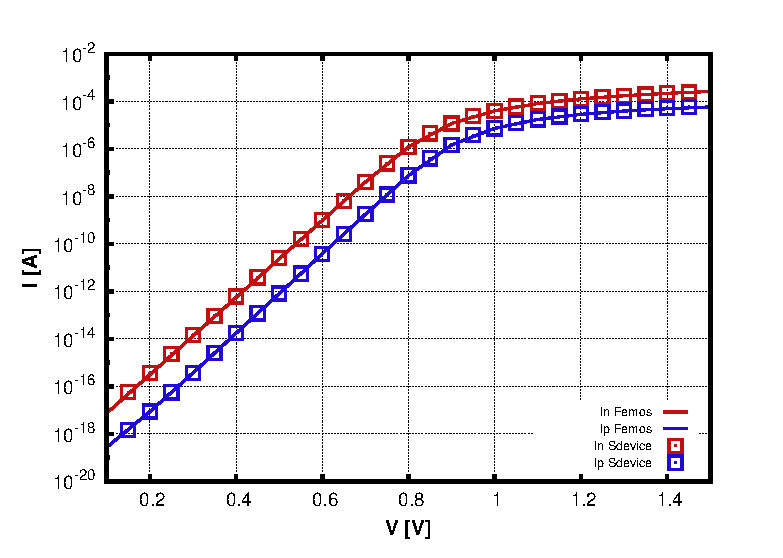
\includegraphics[scale=0.8]{Results/Caratteristiche/DiodeOx/CurrentDiodeOxide.eps}
\caption{Direct polarization constant mobility.}
\end{figure}



\begin{figure}[!h]
\centering
\includegraphics[scale=0.8]{Results/Caratteristiche/DiodeOx/CurrentDiodeOxideMasetti.eps}
\caption{Direct polarization Masetti mobility.}
\end{figure}

\begin{figure}[!h]
\centering
\includegraphics[scale=0.8]{Results/Caratteristiche/DiodeOx/CurrentDiodeOxideConstantVsMasetti.eps}
\caption{Masetti mobility effect Vs. constant mobility effect.}
\end{figure}

Commenti sull'abbassamento della corrente di contatto dovuto all'abbassamento della mobilità

Polarizzazione diretta mobilità canali (??) viene qualitativamente non \`e allineato con sedevice



\clearpage

\subsubsection{MOS n-channel}

Polarizzazion diretta (OK)

Polarizzazione diretta masetti 

Polarizzazione inversa

Stress region contributio impact ionization

Mos acceso mobilità con Velocità di saturazione (??)

\begin{figure}[!h]
\includegraphics[scale=1]{CaratteristicheIV/MOS_Nchannel_191719_DIFFERENTMODELS}
\end{figure}
